\documentclass{article}
\usepackage{graphicx} % Required for inserting images
\usepackage{listings}
\usepackage{xcolor}
\usepackage{tabularx} % Add this in your LaTeX preamble
\usepackage{hyperref}

\lstset{
  basicstyle=\ttfamily\small,
  keywordstyle=\color{blue},
  commentstyle=\color{gray},
  stringstyle=\color{green!60!black},
  showstringspaces=false,
  frame=single,
  breaklines=true,
  captionpos=b
}


\title{PPO Agent for Dicewars}
\author{Eleni Koumparidou\\ Natalia Anastasia Kousta\\
\textbf{Machine Learning}}
\date{April 2025}

\begin{document}

\maketitle

\section{Description}
This project presents the implementation of an AI agent for the game Dicewars using Reinforcement Learning. The report aims to analyze the chosen RL method, describe the implementation of the agent, assess its performance, and propose potential improvements.

\section{Proximal Policy Optimization (PPO)}
The Reinforcement Learning algorithm that we used to implement our player was a policy gradient method, the \textbf{Proximal Policy Optimization (PPO)}. PPO improves the learning progress during training, providing more stable policy upgrades while preventing any performance collapse.

\subsection{Learning process}
The learning process of the PPO agent is based on two neural networks:

\begin{itemize}
    \item \textbf{Policy Network}: It is used to improve the player's policy by providing a probability distribution over possible actions given a state.
    
    \item \textbf{Value Network}: Estimates the expected cumulative future reward from a given state (Value function). This helps the agent to assess how good or bad an action was.
\end{itemize}

\subsection{Learning Optimization}
The agent optimizes the policy using a clipped objective function for small updates and the prediction of future rewards using the Mean Squared Loss (MSE).
All the formulas used for the optimization of the networks are provided bellow:
\begin{itemize}
\item \begin{equation}
L_{actor}(\theta) = \hat{\mathbb{E}}_t \left[ \min\left( r_t(\theta)\hat{A}_t, \text{clip}(r_t(\theta), 1 - \epsilon, 1 + \epsilon) \hat{A}_t \right) \right]
\end{equation}

\item \begin{equation}
\mathcal{L}_{\text{critic}} = \frac{1}{N} \sum_{i=1}^{N} \left( V(s_i) - \hat{R}_i \right)^2
\end{equation}

\item \begin{equation}
A_t = \sum_{l=0}^{\infty} (\gamma \lambda)^l \delta_{t+l}
\end{equation}

\item \begin{equation}
\delta_t = r_t + \gamma V(s_{t+1}) - V(s_t)
\end{equation}

\end{itemize}

Where:
\begin{itemize}
    \item \( r_t(\theta) = \frac{\pi_\theta(a_t | s_t)}{\pi_{\theta_{\text{old}}}(a_t | s_t)} \) is the probability ratio between the new and old policy.
    \item \( \hat{A}_t \) is the estimated \textbf{advantage function}, measuring how much better an action is performed compared to the average.
    \item \( \epsilon \) is a hyperparameter that controls the allowed deviation from the old policy.
    \item $\gamma$: discount factor
    \item $\delta_t$: Temporal Difference (TD) error at current state t
    \item $\lambda$: GAE parameter for bias-variance tradeoff
    \item $r_t$: reward at current state t
    \item $V(s_t)$: Value estimation at current state t
    \item $V(s_{t+1})$: Value estimation at next state t+1
\end{itemize}


\subsection{State Representation for Learning}
We carefully selected the following state information to provide the agent with meaningful inputs that support effective training, while avoiding unnecessary or redundant data that could mislead learning.

\begin{itemize}
    \item \textbf{Number of dice per neighboring area:} The number of dice that every neighbouring area to our player has. We decided to focus only on the neighbours so that the player can decide on a more beneficial action.
    \item \textbf{Number of dice per player:} The total number of dice each player has at the current state.
    \item \textbf{Number of areas per player:} The number of areas each player has at the current state.
    \item \textbf{Maximum cluster per player:} The size of the largest cluster each player has.
    \item \textbf{Number of stocks per player:} The number of stocks each player has.
\end{itemize}


\subsection{Reward function}
Another crucial feature for our agent's efficient learning is the reward function. In order to motivate our agent's learning progress we implemented a reward function that provides positive or negative rewards based on the result that each action has on the parameters used for the state input. So, different small positive rewards are given when the player increases the number of areas, dice or stocks and a large reward in case of winning.  

\section{Implementation Overview}



\subsection{Overview of Core Functions}
A brief description of the functions used in our agent and player is provided in Table \ref{tab:ppo-functions} and Table \ref{tab:player-functions}.

\begin{table}[h]
\centering
\begin{tabularx}{\textwidth}{l X}
\textbf{Function} & \textbf{Description} \\
\hline
\texttt{\_\_init\_\_} & Initializes the PPO agent by setting the necessary parameters for training. \\
\texttt{build\_actor} & Builds the policy (actor) neural network. \\
\texttt{build\_critic} & Builds the value estimation (critic) neural network. \\
\texttt{compute\_advantage} & Computes the advantage function used for policy updates. \\
\texttt{train} & Trains the agent using collected experiences from the games. \\
\texttt{run} & Runs the full training process by initializing and executing multiple games. \\
\texttt{state\_descriptor} & Converts the current environment state into the training format. \\
\texttt{get\_attack\_areas} & Chooses a valid attack by calling \texttt{select\_action}. \\
\texttt{select\_action} & Selects an action using the policy network and epsilon-greedy strategy. \\
\texttt{get\_reward} & Calculates the reward based on the current state. \\
\texttt{save\_model\_weights} & Saves the trained weights of the model for future use. \\
\texttt{training\_plots} & Generates and saves plots to help track training performance. \\
\end{tabularx}
\caption{Descriptions of main functions in the PPO agent class}
\label{tab:ppo-functions}
\end{table}

\begin{table}[h]
\centering
\begin{tabularx}{\textwidth}{l X}
\textbf{Function} & \textbf{Description} \\
\hline
\texttt{\_\_init\_\_} & Initializes the Player with the PPO agent, either by loading pre-trained weights or by training from scratch. \\
\texttt{load\_model\_weights} & Loads the pre-trained weights for the PPO agent. \\
\texttt{get\_attack\_areas} & Selects a valid attack based on the trained Policy network. \\
\end{tabularx}
\caption{Descriptions of main functions in the \texttt{Player} class}
\label{tab:player-functions}
\end{table}




\subsection{Policy and Value Networks}
We implemented the Policy and Value networks (Actor and Critic) using the TensorFlow library, as seen in Listing \ref{lst:networks}. Each neural network consists of four layers, including two hidden layers with 256 nodes each and ReLU activation functions. The output layer of the Policy network uses a softmax activation function to produce a probability distribution over actions. To prevent overfitting, we applied L2 regularization and we used the Adam optimizer for updating the network weights during training.
\\
\begin{lstlisting}[language=Python, caption={Actor and Critic Networks}, label={lst:networks}]
def build_actor(self):
#...
    inputs = Input(shape=(self.state_dim,))     
    x = Dense(256, activation='relu', kernel_regularizer=l2(1e-4))(inputs)  # for overfitting
    x = Dense(256, activation='relu')(x)
    outputs = Dense(self.num_possible_grid_actions, activation='softmax')(x) # Probabilities distribution

    return Model(inputs, outputs)

def build_critic(self):
    #...
    inputs = Input(shape=(self.state_dim,))
    x = Dense(256, activation='relu', kernel_regularizer=l2(1e-4))(inputs)
    x = Dense(256, activation='relu')(x)
    outputs = Dense(1, activation=None)(x)  # Value estimation

    return Model(inputs, outputs)
\end{lstlisting}


\subsection{Reward Function}

We implemented the \texttt{get\_reward} method to give rewards to the agent based on the game state following each action, as described before. After testing the effectiveness of different reward combinations, we decided to provide small positive rewards for beneficial outcomes, while emphasizing on territorial expansion. To encourage this behavior, area conquest is rewarded with a larger scaled value (multiplied by 0.1). Additionally, a significantly larger reward (+10) is given when the player wins the game to motivate strategies that lead to victory.
\\
\begin{lstlisting}[language=Python, caption={Reward function}, label={lst:reward_func}]
def get_reward(self, state, next_state):
    """
    Gives a reward based on the current and the next state
    """
    reward = 0.0

    # Rewards criteria
    area_diff = next_state.player_num_areas[0] - state.player_num_areas[0]  # number of areas 
    dice_diff = next_state.player_num_dice[0] - state.player_num_dice[0]    # number of dice 
    stock_diff = next_state.player_num_stock[0] - state.player_num_stock[0] # number of stock dice

    reward += 1.0 * area_diff
    reward += 0.05 * dice_diff
    reward += 0.05 * stock_diff

    if state.winner == 0:   # Big reward when agent wins
        reward += 10.0

    return reward
\end{lstlisting}

\subsection{State Representation}

To adapt the current game state for learning purposes, we created a descriptor called \texttt{state\_descriptor}. The selected state features are those outlined in the "Input of Learning" chapter. 

First, we identify the neighboring areas of the player. Then, using a helper mask array, we construct an array that contains the number of dice for each neighboring area, while assigning zeros to all non-neighboring areas, so that the agent can focus on the information that are important for the next move. Then we add all the other state features to the state array.
\\
\begin{lstlisting}[language=Python, caption={State Descriptor}, label={lst:descriptor}]
def state_descriptor(self, grid, state):
    #...

    # DICES OF NEIGHBOURS
    neighbours_states = []
    neighbours_areas = []

    # Find the areas that are neighbours of the player's areas
    for area in state.player_areas[0]:
        neighbours_areas.extend(grid.areas[area].neighbors)

    # List of neighbouring areas
    neighbours_areas = list(set(neighbours_areas))  # Keep unique indices

    # Mask for neighbours
    mask = np.zeros_like(state.area_num_dice, dtype=np.float32)
    mask[neighbours_areas] = 1

    area_num_dice = np.array(state.area_num_dice, dtype=np.float32)
    num_dice_neighbours = area_num_dice * mask  # Get neighbour's dices


    #...      
    # Create the state list
    neighbours_states.append(num_dice_neighbours)   # Number of neighbour's dices ---> Length = 30
    neighbours_states.append(player_dices)          # Number of dices per player ---> Length = 4
    neighbours_states.append(player_areas_flat)     # Number of areas per player ---> Length = 4
    neighbours_states.append(player_max_size)       # Size of largest cluster per player ---> Length = 4
    neighbours_states.append(player_num_stock)      # Number of stock dices per player ---> Length = 4

    # Concatenate all features into a single array
    state_features = np.concatenate([np.atleast_1d(feature) for feature in neighbours_states]).astype(np.float32)

    return state_features
\end{lstlisting}

\subsection{Action Selection}
Our agent attacks with \texttt{get\_attack\_areas} and selects an action with \texttt{select\_action}. An action is selected based on the \textbf{Greedy-Epsilon} strategy. This means that the agent chooses a random action with probability $\epsilon$ to encourage exploration of less frequently chosen strategies. This helps discover potentially valuable actions that may not be currently favored by the policy. Otherwise, the agent selects the action with the highest probability, as predicted by the actor network, to exploit known optimal behavior. 


\subsection{Training details}
We train the agent using two main functions, \texttt{run} and  \texttt{train}. The first one executes the training by playing a pre-defined number of games (\texttt{episodes}) and the second one trains the agent after a pre-defined number of finished games (\texttt{train\_freq}). While playing the game the agent collects experience (states, actions, rewards, probabilities) and when the training comes, a random batch of the training experience is selected to train the agent.


\section{Training Evaluation and Performance}
The training parameters are available in Table \ref{tab:train}.

\begin{table}[h]
\centering
\begin{tabular}{l l}
\textbf{Hyperparameter} & \textbf{Value} \\
\hline
Actor learning rate & \texttt{lr\_actor = 0.0003} \\
Critic learning rate & \texttt{lr\_critic = 0.0001} \\
Discount factor & \texttt{gamma = 0.99} \\
Clipping parameter & \texttt{epsilon = 0.4} \\
Exploration parameter & \texttt{e\_explore = 0.6} \\
Minimum exploration value & \texttt{e\_min = 0.1} \\
Exploration decay rate & \texttt{e\_decay = 0.99} \\
Number of games (episodes) & \texttt{episodes = 2000} \\
Training frequency & \texttt{train\_freq = 20} \\
\end{tabular}
\caption{Hyperparameters used for training the PPO agent}
\label{tab:train}
\end{table}


The player was trained against Random Players, achieving an average winning rate of approximately 0.30\% during training. The winning rate of the trained model evaluated before the tournament was 0.305\%, while its performance during the tournament—against three Random Players over 1000 games—dropped to 0.18\%. These results indicate that the overall performance of our agent remains relatively low.

\subsection{Actor Loss Evaluation}

In Figure \ref{fig:actor}, we observe that the actor loss remains relatively stable during the initial training sessions. However, as training progresses, the loss begins to fluctuate significantly, particularly toward the final episodes. Moreover, there is no evident downward trend throughout the training process.

\begin{figure}[h!]
    \centering
    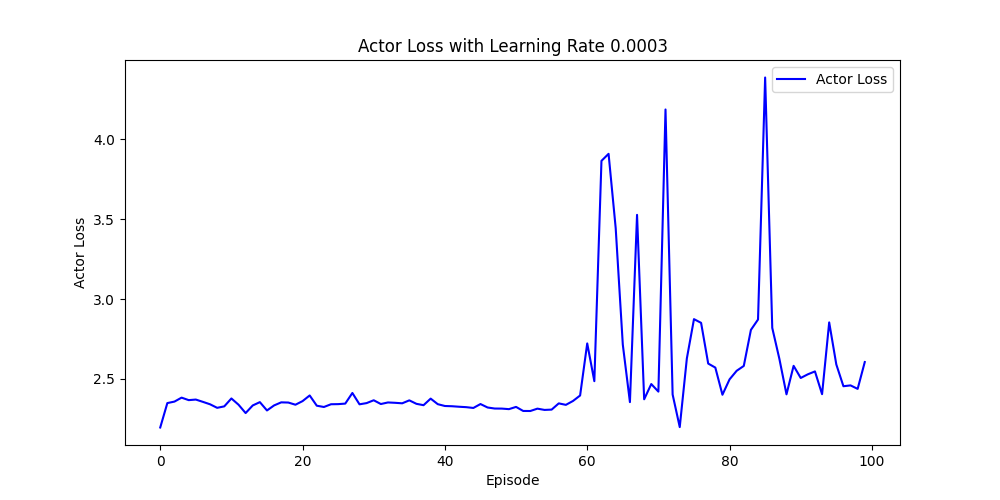
\includegraphics[width=1\linewidth]{assets/actor.png}
    \caption{Actor loss function}
    \label{fig:actor}
\end{figure}

\subsection{Critic Loss Evaluation}

In Figure \ref{fig:critic}, we observe that the critic loss reaches lower values and demonstrates greater stability compared to the actor loss. While occasional drops in the critic loss are noticeable, there is no consistent decreasing trend over time. This could indicate that the value estimates are not progressively improving.

\begin{figure}[h!]
    \centering
    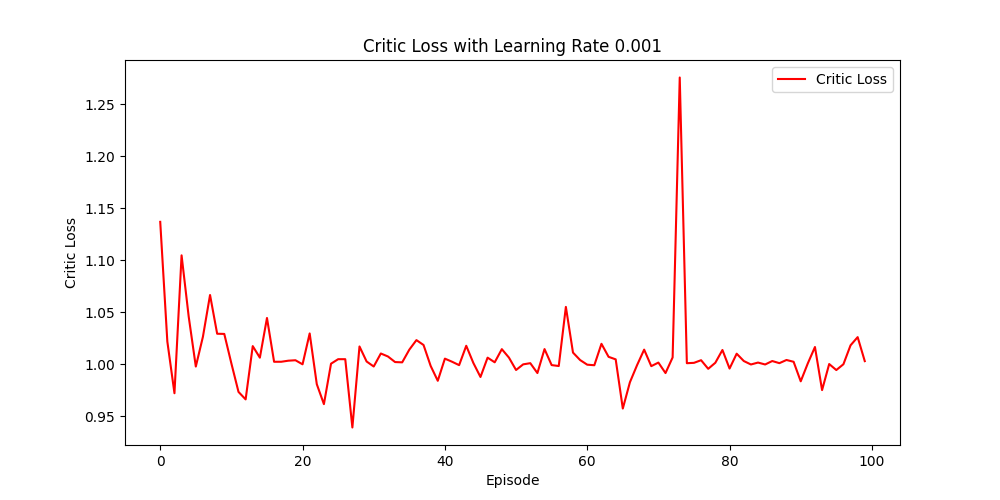
\includegraphics[width=1\linewidth]{assets/critic.png}
    \caption{Critic loss function}
    \label{fig:critic}
\end{figure}

\subsection{Rewards Evaluation}

Figure \ref{fig:rewards} shows the total rewards obtained in each episode during training. Although the agent manages to achieve high rewards at certain points, the overall trend does not show consistent improvement over time. 

\begin{figure}[h!]
    \centering
    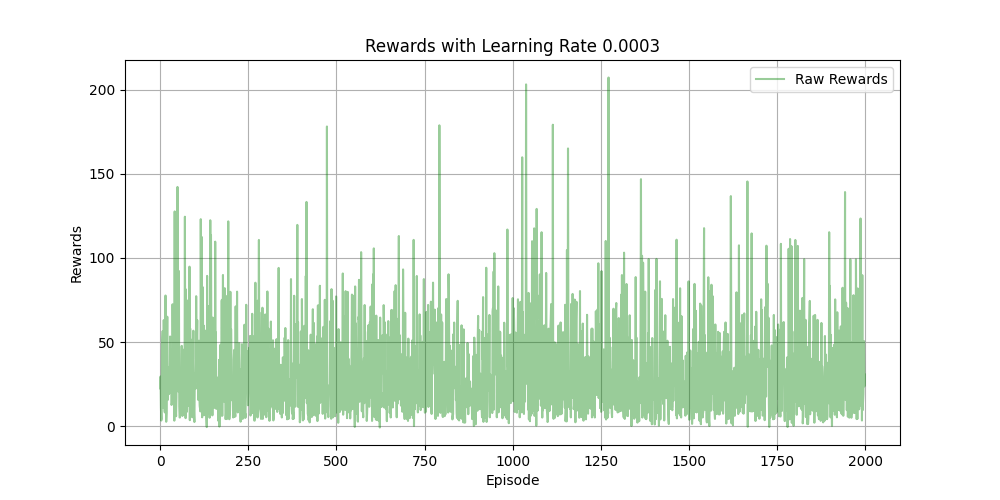
\includegraphics[width=1\linewidth]{assets/rewards.png}
    \caption{Rewards during training}
    \label{fig:rewards}
\end{figure}

\newpage
\section{Improvements}
The evaluation of the training and the performance of our player highlight opportunities for further optimization and improvement. We provide some suggestions that may enhance the learning procedure :

\begin{itemize}
    \item \textbf{Reward Function Adjustment}:  
    
    It is possible that the current reward function does not provide sufficient or consistent feedback to effectively guide the agent during training. One potential improvement is to adjust the scaling parameters of the reward function. Increasing the reward magnitude could make the objective more explicit. Alternatively, reducing the reward scale may provide more stable learning.

    \item \textbf{Training Enhancement}:  

    Another way to improve our agent's learning is by intensifying the training process. This can be achieved by increasing the number of training episodes, for example, extending it to 5.000, or by retraining the agent after the initial training phase to refine its previously learned weights. Additionally, in later training stages, the agent could be trained against more diverse opponents instead of only a Random Player. This would encourage the development of more powerful strategies.

    \item \textbf{Input State Adjustment}: 

    We can also adjust the input state of the training, adding more features of the current state that may be helpful for a more meaningful learning procedure.

    \item \textbf{Hyperparameter Optimization}:

    While we conducted extensive tests to identify the optimal hyperparameters for the training procedure, it is possible that other combinations could further enhance the learning process of our agent.

    
    


    
\end{itemize}


\end{document}
